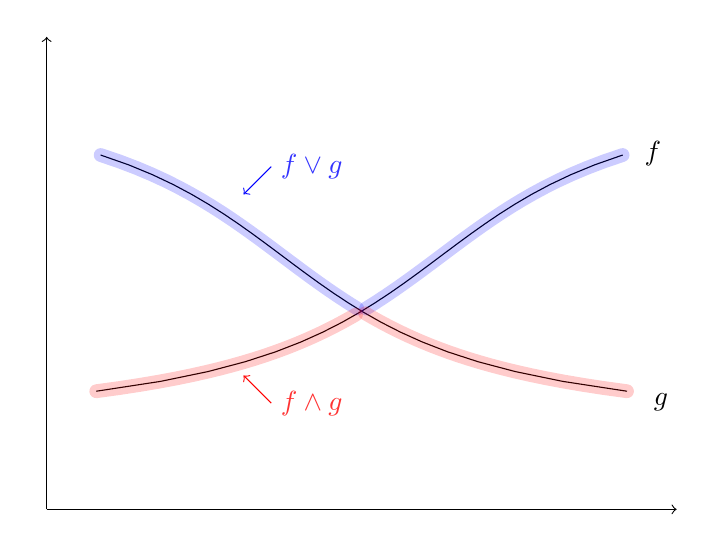
\begin{tikzpicture}

% horizontal 
\draw[->] (0,0) -- (8,0) node[anchor=north] { };

% vertical
\draw[->] (0,0) -- (0,6) node[anchor=east] {};



\draw [black, domain=2:4] plot ({2 * tan(deg(\x)) + 5}, 1.5 * \x - 1.5);
\draw [black, domain=2:4] plot ({2 * tan(deg(-\x)) + 3}, 1.5 * \x - 1.5);

\draw [blue, 
       line width=5pt, 
       domain=2.7:4,
       line cap=round, 
       opacity=0.2] 
       plot ({2 * tan(deg(\x)) + 5}, 1.5 * \x - 1.5);
       
\draw [blue, 
		line width=5pt, 
		domain=2.7:4,
		line cap=round, 
		opacity=0.2] 
		plot ({2 * tan(deg(-\x)) + 3}, 1.5 * \x - 1.5);
       
\draw [red, 
		line width=5pt, 
		domain=2:2.66,
		line cap=round, 
		opacity=0.2] 
		plot ({2 * tan(deg(-\x)) + 3}, 1.5 * \x - 1.5);
		
\draw [red, 
		line width=5pt, 
		domain=2:2.65,
		line cap=round, 
		opacity=0.2] 
		plot ({2 * tan(deg(\x)) + 5}, 1.5 * \x - 1.5);

		 
\draw(7.7,4.8) node[anchor=north] {$f$}
      (7.8,1.6) node[anchor=north] {$g$};
      
\draw [<-, Blue] (2.5,4)-- +(10pt,10pt) node[right, text=blue, opacity=0.8] {$f \vee g$};
\draw [<-, Red] (2.5,1.7)-- +(10pt,-10pt) node[right, text=Red, opacity=0.8] {$f \wedge g$};
		     

		     
\end{tikzpicture}
